\documentclass[11pt,notitlepage]{article}
\usepackage[a4paper, margin={2cm, 2.2cm}]{geometry}
\usepackage[a-2b]{pdfx}[2018/12/22]
\usepackage{alltt, fancyvrb, url}
\usepackage{graphicx}
\usepackage[utf8]{inputenc}
\usepackage{float}
\usepackage{hyperref}
\usepackage{subcaption}
\usepackage{numprint}
\usepackage{slashbox}
\usepackage{pgfplots}
\usepackage{amsmath}
\usepackage{lipsum}
\usepackage{tikz}
\pgfplotsset{compat=1.9,
            tick label style={font=\tiny},
            label style={font=\tiny}}

% Questo commentalo se vuoi scrivere in inglese.
\usepackage[italian]{babel}

\usepackage[italian]{cleveref}

\title{Programmazione concorrente e distribuita \\ Assignment 02}

\author{
    \href{mailto:nicolo.guerra@studio.unibo.it}{Nicolò Guerra, matricola 0001179571} \\
    \href{mailto:filippo.casadei9@studio.unibo.it}{Filippo Casadei, matricola 0001179572} \\
    \href{mailto:emma.leonardi2@studio.unibo.it}{Emma Leonardi, matricola 0001193227}
    }
\date{\today}

\begin{document}
\maketitle
\renewcommand{\thesection}{\arabic{section}}
\section{Analisi del problema}

L'assignment riguarda la creazione di due artefatti differenti: una libreria per la ricerca asincrona di dipendenze in classi, package e progetti Java e una applicazione
reattiva per la visualizzazione delle dipendenze di progetti Java.

\section{Versione asincrona}
%//TODO: scrivere meglio parte di analisi del problema
Il problema principale della versione asincrona riguarda l'accesso in lettura ai file \texttt{.java}, in particolare è importante che le letture da file non blocchino 
il sistema e che vengano eseguite concorrentemente per evitare di bloccare il flusso principale del programma.

Per l'implementazione della libreria è stato utilizzato il framework \texttt{Vertx} che offre supporto alla creazione di sistemi asincroni. In particolare la libreria è formata 
da un oggetto \texttt{DependencyAnalyzer} che si occupa di analizzare i file \texttt{.java} e di restituire le dipendenze in modo asincrono. Fornisce tre metodi principali:
\begin{itemize}
    \item \texttt{getClassDependencies}: cerca le dipendenze di una classe
    \item \texttt{getPackageDependencies}: cerca le dipendenze che le classi di un package hanno verso tipi esterni ad esso
    \item \texttt{getProjectDependencies}: cerca le dipendenze che le classi di un progetto hanno verso tipi esterni ad esso
\end{itemize}
Ogni metodo ritorna un Future generico sul tipo di report che il metodo produce.

La ricerca per le classi è stata implementata utilizzando i metodi di accesso al filesystem messi a disposizione dall'oggetto \texttt{FileSystem} di Vertx, che 
permette di eseguire operazioni non bloccanti, e concatenando a queste le operazioni di parsing e analisi dei file.

Trattandosi di una libreria non sappiamo a priori il contesto all'interno del quale verrà eseguito il codice, per questo abbiamo deciso di non effettuare il deploy di
un oggetto \texttt{Verticle} ma di lasciare la scelta all'utente. Questo da flessibilità alla libreria ma non permette di sapere a priori quale istanza di Vertx verrà utilizzata.
Per questo abbiamo lasciato la possibilità di passare un oggetto \texttt{Vertx} al costruttore dell'oggetto, nel caso in cui questo non venga fatto e venga utilizzato il costruttore
di default, si cerca di recuperare l'oggetto \texttt{Vertx} corrente tramite il metodo \texttt{Vertx.currentContext()} e infine se non esiste un contesto corrente si crea un nuovo
oggetto con chiamata a \texttt{Vertx.vertx()}.

Per i package e i progetti è stato necessario implementare un metodo di ricerca ricorsiva che, partendo dalla directory principale del progetto, analizza i file \texttt{.java}
raccogliendo con un \texttt{Future.all} i risultati asincroni dell'analisi delle classi e dei sotto-package.

Per evitare di fornire risultati parziali e quindi incorretti qualunque problema durante l'analisi di un file \texttt{.java} causa il fallimento dell'intera operazione 
e quindi del relativo \texttt{Future}.

\subsection{Rete di Petri}

\begin{figure}[H]
    \centering
    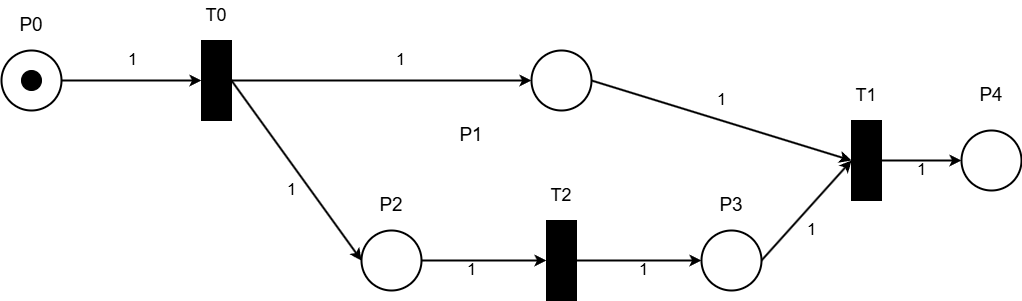
\includegraphics[width=0.7\textwidth]{Petri_async.png}
    \caption{Petri net per la versione asincrona}
    \label{fig:rete-petri-asincrona}
\end{figure}

La rete di Petri per la versione asincrona è composta da una piazza iniziale che rappresenta l'inizio dell'analisi, da qui la transizione \texttt{T0} avvia l'analisi della classe
che prosegue asincronicamente nella piazza \texttt{P2}, mentre il main prosegue in \texttt{P1} e continua con la sua computazione. Una volta completata l'analisi 
(transizione \texttt{T2}) il risultato è pronto per essere gestito (piazza \texttt{P3}) e viene gestito nella transizione \texttt{T1} che porta alla conclusione 
della computazione asincrona (piazza \texttt{P4}).

\subsection{Utilizzo versione asincrona}
Per provare la versione asincrona è necessario avviare il metodo main della classe \texttt{pcd.ass02.async.VertxApp} con i parametri:
\begin{itemize}
    \item \texttt{--class [class file path]}: per analizzare una singola classe
    \item \texttt{--package [package folder path]}: per analizzare un package
    \item \texttt{--project [project folder path]}: per analizzare un progetto
\end{itemize}

\section{Versione reattiva}
Mentre nell'approccio asincrono il main si preoccupa di mettere in coda delle task da eseguire e di gestire il loro completamento (o fallimento) in qualche modo, 
l'approccio reattivo si differenzia nel fatto che si ha un componente osservabile che continua a eseguire in background e il flusso principale del programma deve 
occuparsi di reagire in qualche modo agli eventi che questo osservabile fa scattare. 

Deve inoltre, essendo i nostri osservabili infiniti, occuparsi di farlo terminare al momento opportuno. L'analisi delle dipendenze in questo caso è perciò affidata 
all'esecuzione di un \texttt{Observable} di tipo cold che istanzia un nuovo thread, questo si occupa al suo avvio di cercare le dipendenze in background nei file 
e inviare un nuovo oggetto dependency ogni volta che ne trova una, una volta esplorati tutti i file il thread si mette in osservazione della cartella di progetto
selezionata per eventuali cambiamenti e in caso di modifiche ai sorgenti li rianalizza e notifica la view del cambiamento che si occupa di aggiornare il grafo, 
permettendo così di reagire in tempo reale a modifiche dei file. 

La ricerca avviene chiamando sull'oggetto \texttt{ReactiveDependencyFinder} il metodo \\
\texttt{findAllClassesDependencies} che restituisce un \texttt{Observable} che emette un oggetto \\
\texttt{ClassDependencyInfo} ogni volta che trova una dipendenza o che una dipendenza già notificata varia.

Il controller mantiene un grafo delle dipendenze come oggetto \texttt{DependenciesGraph} e la view lo disegna (tramite un oggetto wrapper per compatibilità con la libreria grafica)
ogni volta che il controller riceve una notifica di cambiamento dall'observable.

La view è implementata in \texttt{JavaFX} e mostra il grafo delle dipendenze sfruttando la libreria \texttt{JavaFX Smart Graph}\footnote{\url{https://github.com/brunomnsilva/JavaFXSmartGraph}}.
Il grafo è composto da nodi di colore rosso che rappresentano le classi di progetto, nodi di colore blu che rappresentano le classi esterne su cui sono presenti dipendenze e archi orientati
che collegano le classi alle loro dipendenze.

Mostra inoltre le classi totali analizzate e il numero di dipendenze trovate, si può inoltre fermare l'analisi reattiva con un apposito pulsante che causa la
terminazione del thread di analisi e la chiusura dell'osservabile.

\subsection{Rete di Petri}

\begin{figure}[H]
    \centering
    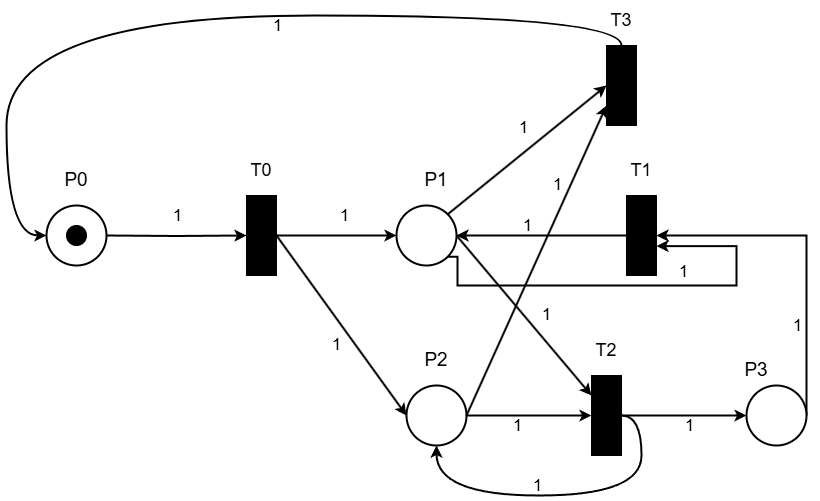
\includegraphics[width=0.7\textwidth]{Petri_reactive.png}
    \caption{Petri net per la versione reattiva}
    \label{fig:rete-petri-reattiva}
\end{figure}

La rete di Petri per la versione reattiva è composta da una piazza iniziale \texttt{P0} che rappresenta l'avvio dell'analisi, da qui la transizione \texttt{T0} avvia l'analisi del progetto
in background. Il main prosegue in \texttt{P1} e continua con le sue computazioni, intanto l'analisi prosegue in \texttt{P2} e quando trova una dipendenza la notifica (transizione \texttt{T2})
alla piazza \texttt{P3}. La transizione T1 rappresenta la gestione dell'evento e l'aggiornamento della view. Infine una volta fermata l'analisi (transizione \texttt{T3}) il thread di analisi 
termina e si ritorna allo stato iniziale (piazza \texttt{P4}) svuotando inoltre la piazza \texttt{P3}.

\subsection{Utilizzo versione reattiva}

Per utilizzare la versione reattiva è necessario avviare il metodo main della classe \\
\texttt{pcd.ass02.reactive.ReactiveApp} e scegliere una cartella di progetto con il tasto \texttt{Select directory}.
A questo punto è possibile avviare l'analisi con il tasto \texttt{Start} e verrà mostrato il grafo delle dipendenze mantenendo l'analisi reattiva fino a quando non si preme 
il tasto \texttt{Stop} o non si chiude il programma.
È inoltre possibile attivare o disattivare l'auto layout del grafo con l'apposita checkbox, effettuare lo zoom utilizzando CTRL+scroll e spostare il grafo con il mouse.

\end{document}
